%%% In this section, you will describe all of the various artifacts that you will generate and maintain during the project life cycle. Describe the purpose of each item below, how the content will be generated, where it will be stored, how often it will be updated, etc. Replace the default text for each section with your own description. Reword this paragraph as appropriate.

\subsection{Major Documentation Deliverables}

\subsubsection{Project Charter}

We will be maintaining this project charter during all sprints. Usually near the end once we get a better understanding of what we have accomplished then update it. The initial version of our project charter will come out once our product has reached testing phase, and the final version will be once we have everything working. 

\subsubsection{System Requirements Specification}

We will be updating System Requirements specifications anytime we have a major change in our project like a shift in languages or hardware. The initial version should come out once we have our finished product and working on distribution. 

\subsubsection{Architectural Design Specification}

This document will be maintained near the end of sprints so we can take a look back and be able to properly explain how we built it. We will have a meeting talking about how we will got about the architectural and compare it to the finally result and check they are the same. This will be delivered along side of the Project Charter so that anyone can see our Design process in understanding what we did.


\subsubsection{Detailed Design Specification}

This document will be maintained alongside the Architectural due to the similarities between the documents. We will be following the same process when we update this document and Architectural Design. 

\subsection{Recurring Sprint Items}



\subsubsection{Product Backlog}

The items will be add to the SRS by when we need to add. The items will be prioritized based on due dates from sponsor and then what can be done within the sprint. Decision are left to a vote when capable. We will be using excel for our product back log. 


\subsubsection{Sprint Planning}

Each sprint, we'll plan on Monday that starts our sprint, then every Friday, we meet together to collaborate. We will also tend to meet on weekends virtually as well for collaboration. We will be having four sprints this semester, and possibly another 4 more sprints for the next semester.

\subsubsection{Sprint Goal}

Our sprint goal is decided by our sponsor currently, and as a group. We will ask friends what they would want from this software for ideas but in the end it is up the group.

\subsubsection{Sprint Backlog}

With the meeting on Friday we will decide what goes onto the sprint back log, and the backlog will be maintained by everyone on excel.

\subsubsection{Task Breakdown}

Everyone will voluntarily claim task and we will document our time on our backlog.

\subsubsection{Sprint Burn Down Charts}

Caleb will be responsible for generating the burn down chart for each sprint. They will take from the backlog and take the time expected to finish all of the work and document each day about how much was done. The format is just a simple line (Red line) from expected effort to 0, and then our document line (blue line) showing what we have done.

\begin{figure}[h!]
    \centering
    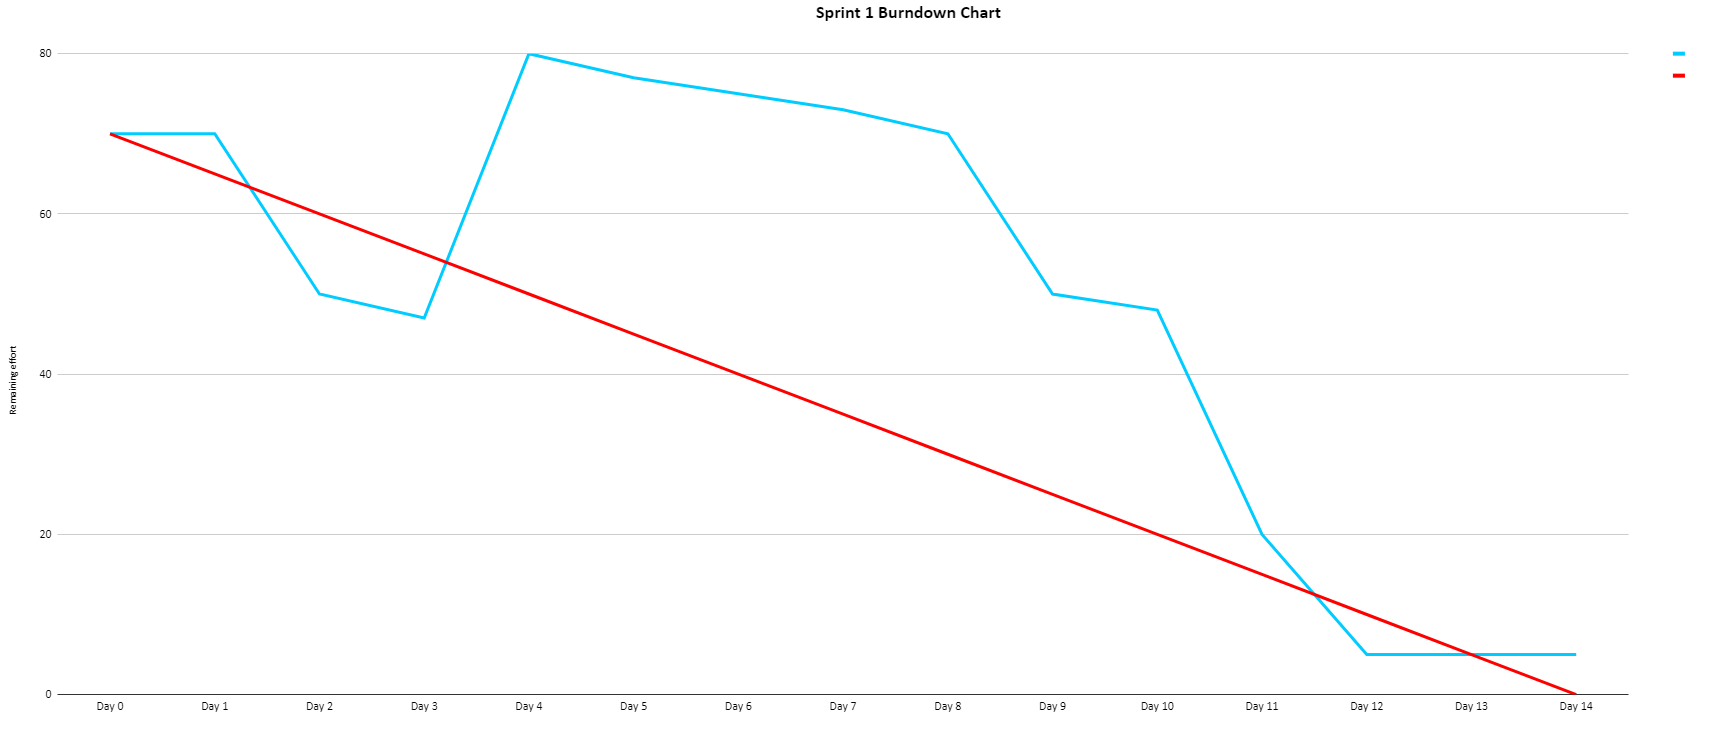
\includegraphics[width=0.8\textwidth]{images/ExampleSprint}
    \caption{Example sprint burn down chart}
\end{figure}

\subsubsection{Sprint Retrospective}

On the Friday, after the sprint is done, we will talk about what has happen. The individual will document what they have done for each task where the group is documented based on the deliverables and documentation. 

\subsubsection{Individual Status Reports}

Everyone will been given the same status up, and it will be reported on after the sprint. The key items is our sprint goals, backlog, Individual time expenditures, team burn down chart, individual retrospectives, and a peer review. 

\subsubsection{Engineering Notebooks}

We do not plan to use an Engineering note book. That is up the the individual if they wish to do that.

\subsection{Closeout Materials}

\subsubsection{System Prototype}

In our final system prototype we expect the have the software being able to have a lesson plan, and sandbox mode. We want the user to be able to learn how to use the ThereMelo within and have fun with it. 


\subsubsection{Project Poster}

The Poster will just be a tri-fold presentation board and it will just have who we are and what are product is. 

\subsubsection{Web Page}

For our web page we would want to post everything and we want it to be accessible to the public. This will be provided at the end once our product is completed. 

\subsubsection{Demo Video}

We will show the process/ behind the scene of the game as B-reel footage while we explain how our software works. The video should only be around 3 minutes and it will just cover how our product works and run a simple lesson. 

\subsubsection{Source Code}

We will be using GitHub as our version control system. We plan to have our software to just be binaries but we would like to also include the source code. The product will be open sourced for the general public at the end and we will be using GNU GPL for our license. It will be all in the LICENSE in main. 

\subsubsection{Source Code Documentation}

We will be using Doxygen and we will have it as a pdf.

\subsubsection{Hardware Schematics}

We do not have any hardware so this is not applicable to us

\subsubsection{CAD files}

We do not have any CAD files so this is not applicable to us

\subsubsection{Installation Scripts}

We will try to use Unity as a way to allow for user to download it. 

\subsubsection{User Manual}

We will create a digital user manual, but it is not likely needed to the program should be able to run as long as the camera and any other software is already downloaded. 